\documentclass[12pt,letterpaper]{article}

\usepackage[utf8]{inputenc}
\usepackage[spanish]{babel}
\usepackage{graphicx}
\usepackage[hidelinks]{hyperref}
\usepackage{hyperref}
\usepackage[left=2cm,right=2cm,top=2.5cm,bottom=2cm]{geometry}
\usepackage{graphicx}
\usepackage{float}
\usepackage{amsmath}
\usepackage{stackrel} 
\usepackage{multicol}
\usepackage{multirow}
\usepackage{fancyhdr}
\usepackage[usenames,dvipsnames,svgnames,table]{xcolor}
\usepackage[document]{ragged2e}
\usepackage{enumerate}

\usepackage{helvet}

\renewcommand{\labelitemi}{$-$}
\renewcommand{\labelitemii}{$\cdot$}
\newcommand\tab[1][1cm]{\hspace*{#1}}

\renewcommand{\familydefault}{\sfdefault}

\definecolor{azul}{RGB}{0,0,255}

\pagestyle{fancy}
\lhead{\begin{picture}(0,0) \put(0,0){
\includegraphics[width=10mm]{./img/logo}} \end{picture}}
\chead{\hspace{1cm}\vspace{0.2cm}Laboratorio 01 - Modelamiento Dimensional}
\rhead{}

\begin{document}
\begin{titlepage}
    \begin{center}
        \begin{figure}[htb]
            \begin{center}
                
\includegraphics[width=3.5cm]{./img/logo}
            \end{center}
        \end{figure}
        \vspace*{0.15in}
        \begin{Large}
            \textbf{UNIVERSIDAD PRIVADA DE TACNA}\\
        \end{Large}
        \vspace*{0.15in}
        \begin{Large}
            \textbf{FACULTAD DE INGENIERÍA} \\
        \end{Large}
        \vspace*{0.1in}
        \begin{Large}
            \textbf{Escuela Profesional de Ingeniería de Sistemas} \\
        \end{Large}
        \vspace*{0.3in}
        \begin{Large}
            \textbf{Laboratorio 01}\\
            \textbf{``Modelamiento Dimensional"}\\
        \end{Large}
        \vspace*{0.2in}
        \begin{Large}
            \textbf{CURSO:} \\
        \end{Large}
        \vspace*{0.1in}
        \begin{large}
            Inteligencia de Negocios\\
        \end{large}
        \vspace*{0.2in}
        \begin{Large}
            \textbf{DOCENTE:} \\
        \end{Large}
        \vspace*{0.1in}
        \begin{large}
            Mag. Patrick Jose Cuadros Quiroga\\
        \end{large}
        \vspace*{0.3in}
        \begin{large}
            \textbf{ALUMNO:} \\
            \begin{flushleft}
                Lipa Calabilla, Abraham  		\hfill	(2019064039) \\
            \end{flushleft}
        \end{large}
        \vspace*{1.3in}
        \begin{large}
            Tacna - Perú\\
        \end{large}
        \vspace*{0.1in}
        \begin{large}
            2022\\
        \end{large}
    \end{center}
\end{titlepage}
\include{Secciones/articulo}
\newpage
\tableofcontents
\justify
\newpage
\begin{LARGE}
    \begin{center}
        \textbf{MODELAMIENTO DIMENSIONAL} \\
    \end{center}
\end{LARGE}
\section{OBJETIVOS}
\begin{itemize}
    \item Aplicar los conceptos de Modelamiento Dimensional
\end{itemize}

\section{REQUERIMIENTOS}
\begin{itemize}
    \item Conocimientos\\
          Para el desarrollo de esta práctica se requerirá de los siguientes conocimientos básicos:
          \begin{itemize}
              \item Conocimientos básicos de administración de base de datos Microsoft SQL Server.
              \item Conocimientos básicos de SQL.
          \end{itemize}
    \item Software\\
          Así mismo se necesitan los siguientes aplicativos:
          \begin{itemize}
              \item Microsoft SQL Server 2016 o superior
              \item Base de datos AdventureWorksDW2016 o superior
          \end{itemize}
\end{itemize}

\section{CONSIDERACIONES INICIALES}
\begin{itemize}
    \item Generar todos los modelos físicos de los diagramas entidad relación y modelo dimensional en bases de datos separadas en Microsoft SQL Server.
\end{itemize}

\newpage
\section{DESARROLLO}
\subsection{Ejercicio N° 01: Envíos}
El siguiente diagrama E / R simplificado describe el envío de mercancías. Los lotes pertenecientes a ciertos grupos se envían a ciertos destinos en varios países a través de diferentes modos de transporte. Un cierto centro de costos es responsable de cada envío. La dimensión de tiempo consiste en mes y año

\begin{center}
    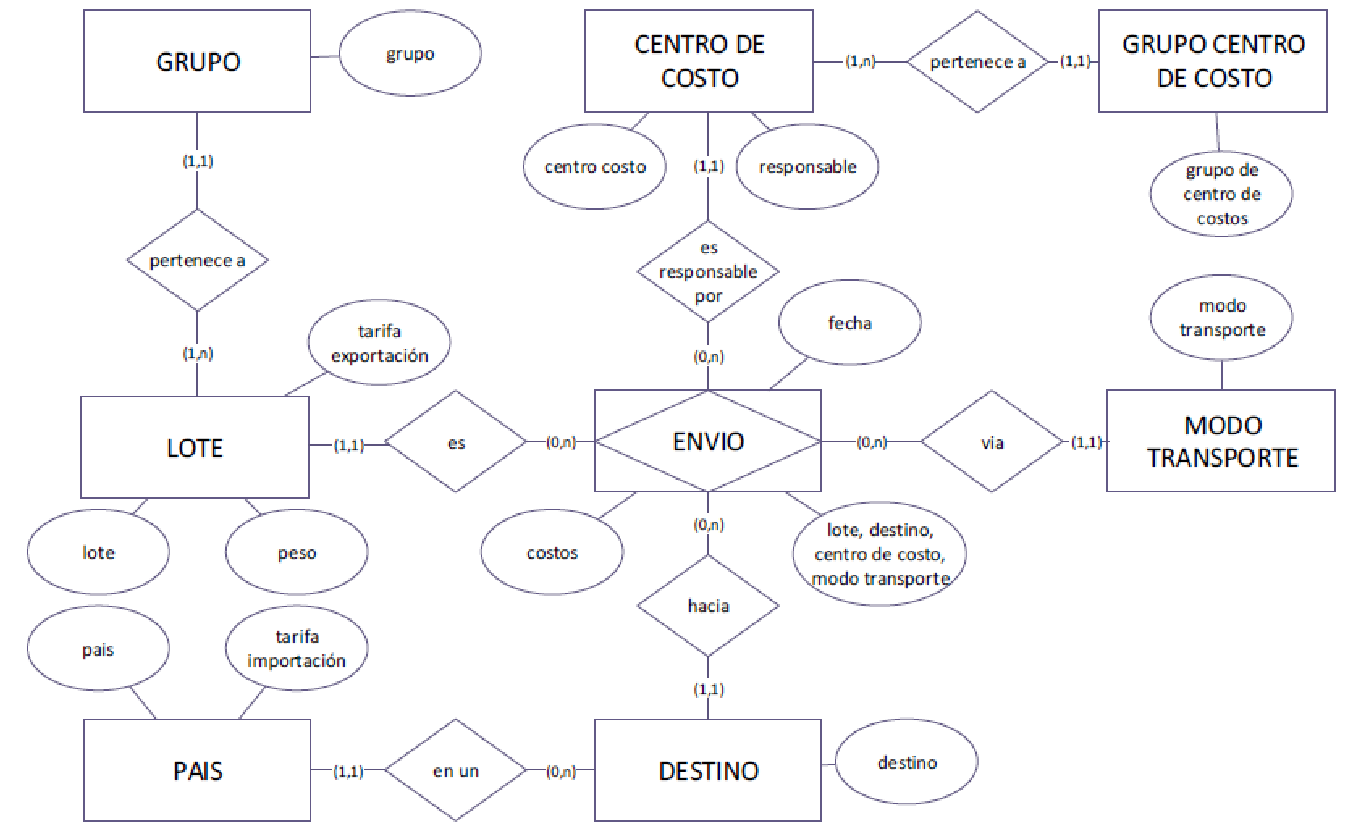
\includegraphics[width=13cm]{./img/img1.png}
\end{center}

Supongamos que los costos de los atributos ya incluyen todas las tarifas. No se transferirá más información sobre las tarifas al almacén de datos. El análisis tendrá lugar a nivel del grupo de centros de costos, no se necesita información sobre los centros de costos.\\

Por favor identifique el hecho de interés y construya el Modelo Dimensional y su respectivo diagrama físico

\begin{enumerate}[\tab a.]
    \item \textbf{Modelo dimensional inicial}
    \begin{center}
        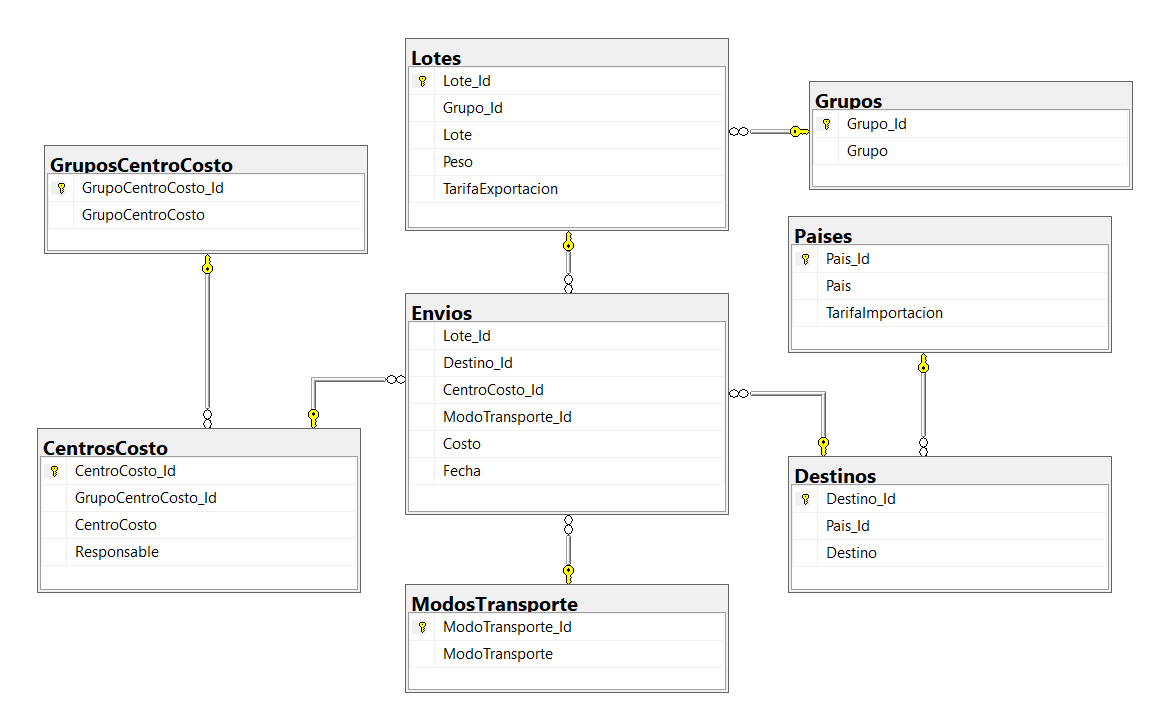
\includegraphics[width=16cm]{./img/img4.png}
    \end{center}
    \subitem Código SQL
    \begin{verbatim}
        CREATE TABLE DIM_Grupos (
            Grupo_Id INT IDENTITY(1,1) PRIMARY KEY,
            Grupo VARCHAR(63)
        );
        CREATE TABLE DIM_Lotes (
            Lote_Id INT IDENTITY(1,1) PRIMARY KEY,
            Grupo_Id INT NOT NULL,
            Lote VARCHAR(63),
            Peso DECIMAL(8,2),
            TarifaExportacion DECIMAL(8,2)
            FOREIGN KEY (Grupo_Id) REFERENCES DIM_Grupos(Grupo_Id)
        );
    
    
        CREATE TABLE DIM_Paises (
            Pais_Id INT IDENTITY(1,1) PRIMARY KEY,
            Pais VARCHAR(63),
            TarifaImportacion DECIMAL(8,2)
        );
        CREATE TABLE DIM_Destinos (
            Destino_Id INT IDENTITY(1,1) PRIMARY KEY,
            Pais_Id INT NOT NULL,
            Destino VARCHAR(63),
            FOREIGN KEY (Pais_Id) REFERENCES DIM_Paises(Pais_Id)
        );
    
    
        CREATE TABLE DIM_GruposCentroCosto (
            GrupoCentroCosto_Id INT IDENTITY(1,1) PRIMARY KEY,
            GrupoCentroCosto VARCHAR(63)
        );
        CREATE TABLE DIM_CentrosCosto (
            CentroCosto_Id INT IDENTITY(1,1) PRIMARY KEY,
            GrupoCentroCosto_Id INT NOT NULL,
            CentroCosto VARCHAR(63),
            Responsable VARCHAR(63),
            FOREIGN KEY (GrupoCentroCosto_Id) REFERENCES DIM_GruposCentroCosto(GrupoCentroCosto_Id)
        );
    
    
        CREATE TABLE DIM_ModosTransporte (
            ModoTransporte_Id INT IDENTITY(1,1) PRIMARY KEY,
            ModoTransporte VARCHAR(63)
        );
    
    
        CREATE TABLE BT_Envios (
            Lote_Id INT NOT NULL,
            Destino_Id INT NOT NULL,
            CentroCosto_Id INT NOT NULL,
            ModoTransporte_Id INT NOT NULL,
            Costos DECIMAL(8,2),
            Fecha DATETIME,
            FOREIGN KEY (Lote_Id) REFERENCES DIM_Lotes(Lote_Id),
            FOREIGN KEY (Destino_Id) REFERENCES DIM_Destinos(Destino_Id),
            FOREIGN KEY (CentroCosto_Id) REFERENCES DIM_CentrosCosto(CentroCosto_Id),
            FOREIGN KEY (ModoTransporte_Id) REFERENCES DIM_ModosTransporte(ModoTransporte_Id),
        );
    \end{verbatim}

    \item \textbf{Modelo dimensional final} (Sin las tablas que no requieren información)
    \begin{center}
        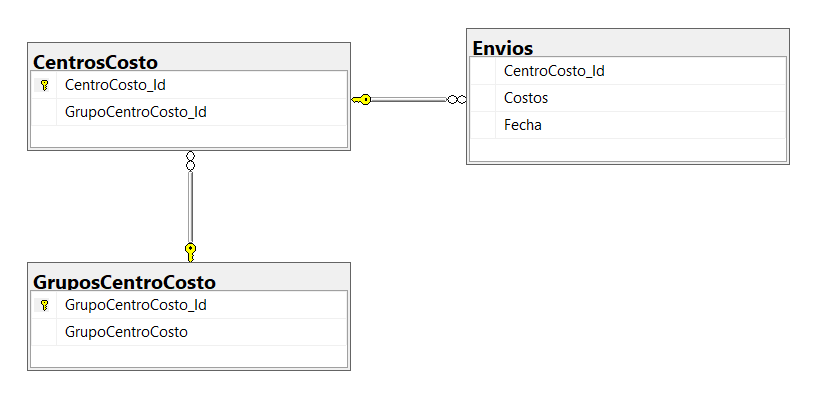
\includegraphics[width=13cm]{./img/img5.png}
    \end{center}
    \subitem Código SQL
    \begin{verbatim}
        CREATE TABLE DIM_GruposCentroCosto (
            GrupoCentroCosto_Id INT IDENTITY(1,1) PRIMARY KEY,
            GrupoCentroCosto VARCHAR(63)
        );
        CREATE TABLE DIM_CentrosCosto (
            CentroCosto_Id INT IDENTITY(1,1) PRIMARY KEY,
            GrupoCentroCosto_Id INT NOT NULL,
            FOREIGN KEY (GrupoCentroCosto_Id) REFERENCES DIM_GruposCentroCosto(GrupoCentroCosto_Id)
        );
    
    
        CREATE TABLE BT_Envios (
            CentroCosto_Id INT NOT NULL,
            Costos DECIMAL(8,2),
            Fecha DATETIME,
            FOREIGN KEY (CentroCosto_Id) REFERENCES DIM_CentrosCosto(CentroCosto_Id),
        );    
    \end{verbatim}
\end{enumerate}

\subsection{Ejercicio N° 02: Reservas de viaje}
En este esquema de E / R, un cliente (que es de cierto tipo) reserva un viaje en una agencia de viajes. La agencia de viajes trabaja para un determinado operador turístico. El viaje va a un destino determinado que pertenece a un país determinado. La dimensión de tiempo consiste en mes, trimestre y año.

\begin{center}
    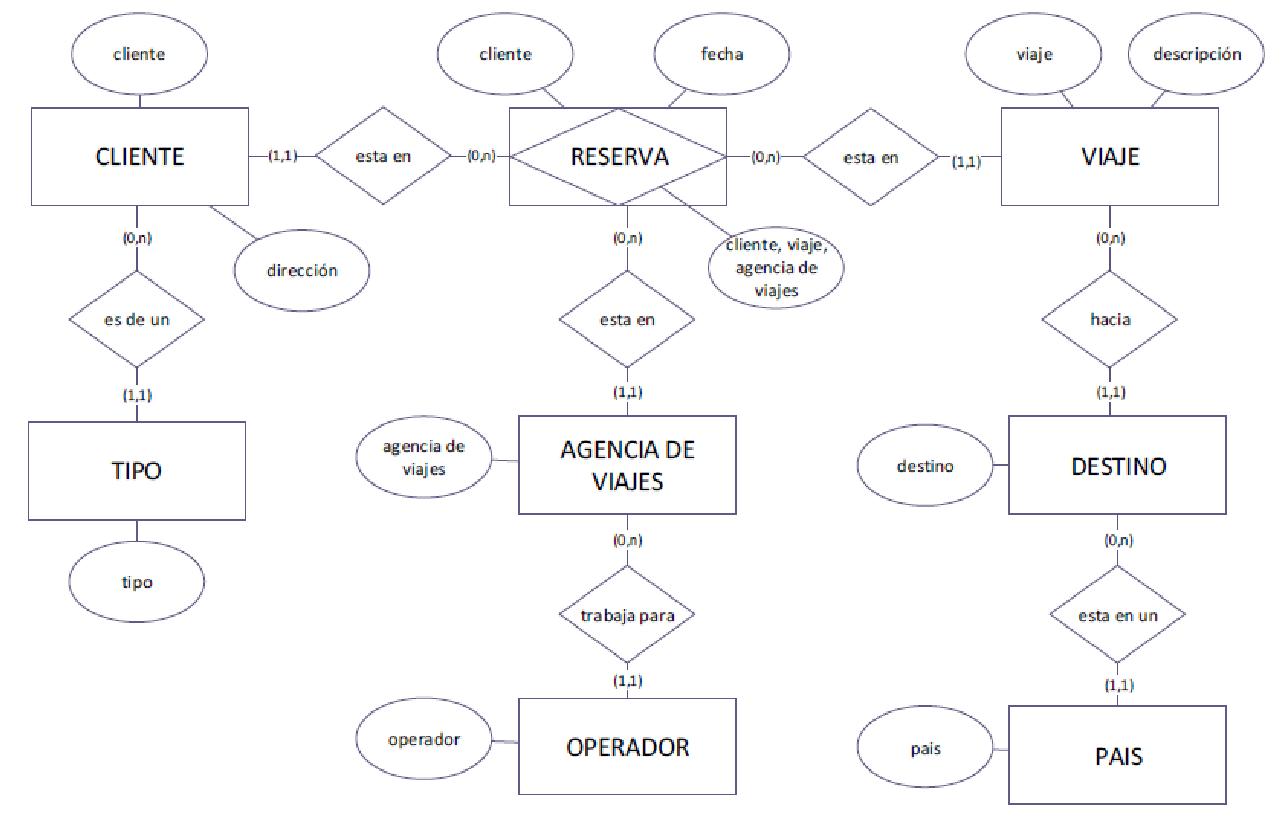
\includegraphics[width=13cm]{./img/img2.png}
\end{center}

Por favor identifique el hecho de interés y construya el Modelo Dimensional y su respectivo esquema físico.

\textbf{Modelo dimensional}
\begin{center}
    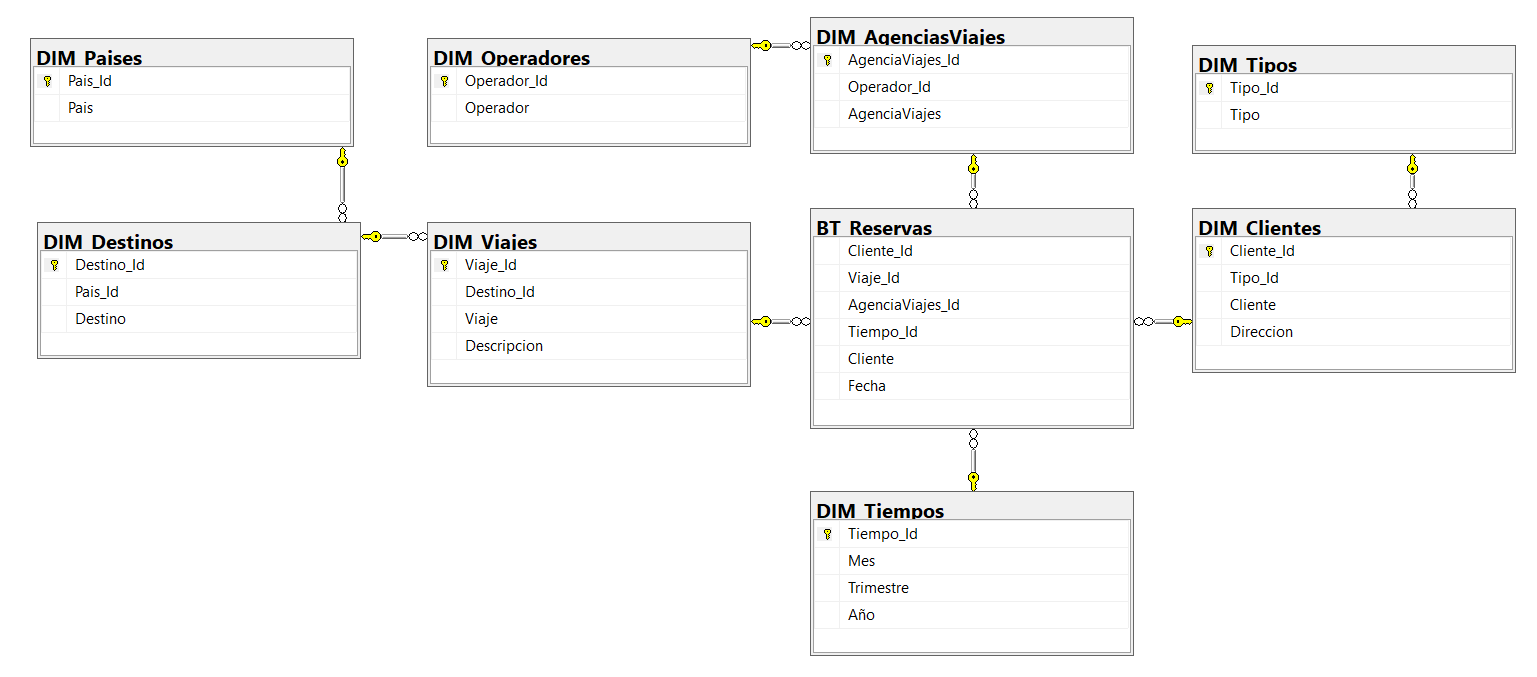
\includegraphics[width=16cm]{./img/img6.png}
\end{center}

Código SQL
\begin{verbatim}
    CREATE TABLE DIM_Tipos (
		Tipo_Id INT IDENTITY(1,1) PRIMARY KEY,
		Tipo VARCHAR(63)
	);
	CREATE TABLE DIM_Clientes (
		Cliente_Id INT IDENTITY(1,1) PRIMARY KEY,
		Tipo_Id INT NOT NULL,
		Cliente VARCHAR(63),
		Direccion VARCHAR(63),
		FOREIGN KEY (Tipo_Id) REFERENCES DIM_Tipos(Tipo_Id)
	);


	CREATE TABLE DIM_Operadores (
		Operador_Id INT IDENTITY(1,1) PRIMARY KEY,
		Operador VARCHAR(63)
	);
	CREATE TABLE DIM_AgenciasViajes (
		AgenciaViajes_Id INT IDENTITY(1,1) PRIMARY KEY,
		Operador_Id INT NOT NULL,
		AgenciaViajes VARCHAR(63),
		FOREIGN KEY (Operador_Id) REFERENCES DIM_Operadores(Operador_Id)
	);


	CREATE TABLE DIM_Paises (
		Pais_Id INT IDENTITY(1,1) PRIMARY KEY,
		Pais VARCHAR(63),
	);
	CREATE TABLE DIM_Destinos (
		Destino_Id INT IDENTITY(1,1) PRIMARY KEY,
		Pais_Id INT NOT NULL,
		Destino VARCHAR(63),
		FOREIGN KEY (Pais_Id) REFERENCES DIM_Paises(Pais_Id)
	);
	CREATE TABLE DIM_Viajes (
		Viaje_Id INT IDENTITY(1,1) PRIMARY KEY,
		Destino_Id INT NOT NULL,
		Viaje VARCHAR(63),
		Descripcion VARCHAR(63),
		FOREIGN KEY (Destino_Id) REFERENCES DIM_Destinos(Destino_Id)
	);


	CREATE TABLE DIM_Tiempos (
		Tiempo_Id INT IDENTITY(1,1) PRIMARY KEY,
		Mes INT,
		Trimestre INT,
		Año INT
	);


	CREATE TABLE BT_Reservas (
		Cliente_Id INT NOT NULL,
		Viaje_Id INT NOT NULL,
		AgenciaViajes_Id INT NOT NULL,
		Tiempo_Id INT NOT NULL,
		Cliente VARCHAR(63),
		Fecha DATETIME,
		FOREIGN KEY (Cliente_Id) REFERENCES DIM_Clientes(Cliente_Id),
		FOREIGN KEY (Viaje_Id) REFERENCES DIM_Viajes(Viaje_Id),
		FOREIGN KEY (AgenciaViajes_Id) REFERENCES DIM_AgenciasViajes(AgenciaViajes_Id),
		FOREIGN KEY (Tiempo_Id) REFERENCES DIM_Tiempos(Tiempo_Id)
	);
\end{verbatim}

\subsection{Ejercicio N° 03: Gestión de proyectos}
Este esquema E / R simplificado muestra un caso gestión del proyecto.\\
El proyecto para un cliente se divide en varios paquetes de trabajo y siempre una persona es responsable de completar la
tarea. Se cuida en un lugar determinado.\\
La dimensión de tiempo consiste de día, mes y año.

\begin{center}
    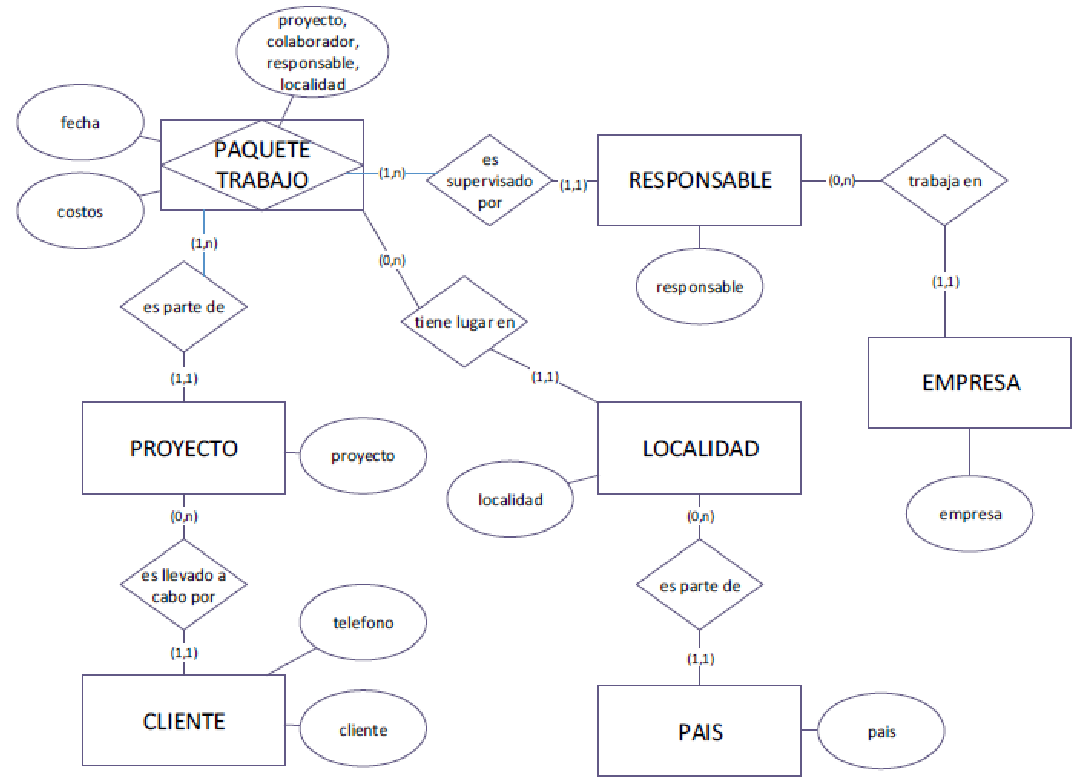
\includegraphics[width=13cm]{./img/img3.png}
\end{center}

Por favor identifique el hecho de interés y construya el Modelo Dimensional. Incluya un atributo de hecho adicional que cuente la cantidad de paquetes de trabajo. Asimismo, realice el diagrama físico.

\textbf{Modelo dimensional}
\begin{center}
    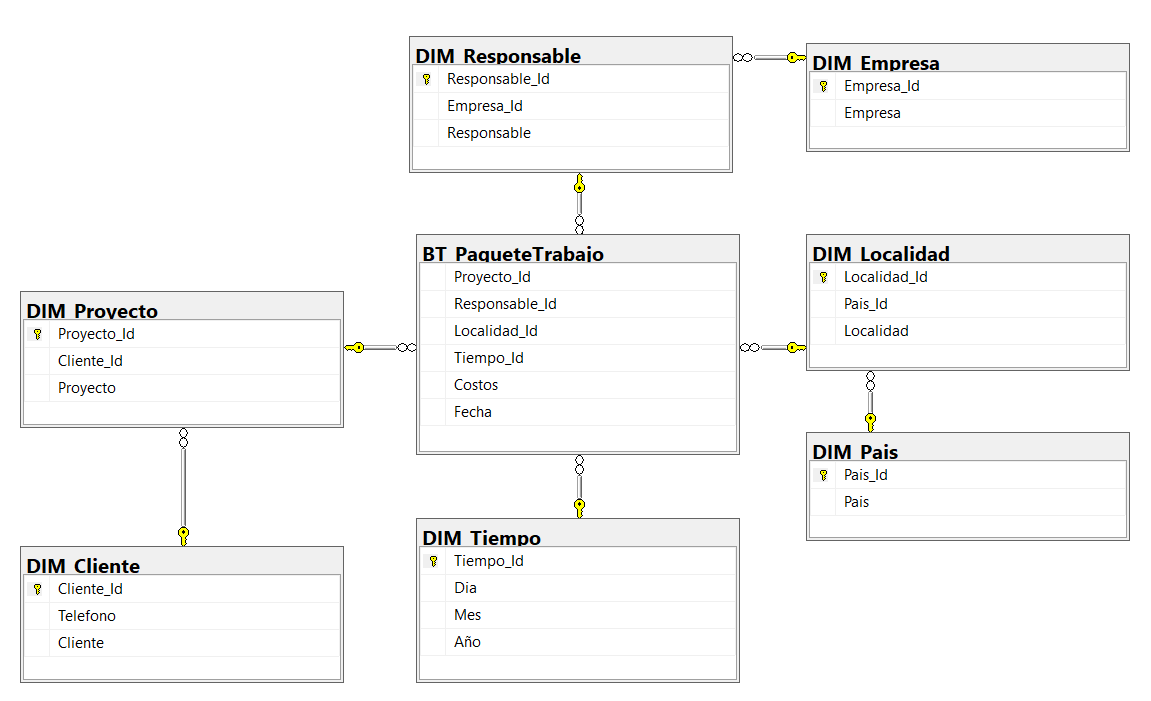
\includegraphics[width=16cm]{./img/img7.png}
\end{center}

Código SQL
\begin{verbatim}
    CREATE TABLE DIM_Cliente (
		Cliente_Id INT IDENTITY(1,1) PRIMARY KEY,
		Telefono VARCHAR(9),
		Cliente VARCHAR(63)
	);
	CREATE TABLE DIM_Proyecto (
		Proyecto_Id INT IDENTITY(1,1) PRIMARY KEY,
		Cliente_Id INT NOT NULL,
		Proyecto VARCHAR(63),
		FOREIGN KEY (Cliente_Id) REFERENCES DIM_Cliente(Cliente_Id)
	);


	CREATE TABLE DIM_Empresa (
		Empresa_Id INT IDENTITY(1,1) PRIMARY KEY,
		Empresa VARCHAR(63)
	);
	CREATE TABLE DIM_Responsable (
		Responsable_Id INT IDENTITY(1,1) PRIMARY KEY,
		Empresa_Id INT NOT NULL,
		Responsable VARCHAR(63),
		FOREIGN KEY (Empresa_Id) REFERENCES DIM_Empresa(Empresa_Id)
	);


	CREATE TABLE DIM_Pais (
		Pais_Id INT IDENTITY(1,1) PRIMARY KEY,
		Pais VARCHAR(63),
	);
	CREATE TABLE DIM_Localidad (
		Localidad_Id INT IDENTITY(1,1) PRIMARY KEY,
		Pais_Id INT NOT NULL,
		Localidad VARCHAR(63),
		FOREIGN KEY (Pais_Id) REFERENCES DIM_Pais(Pais_Id)
	);


	CREATE TABLE DIM_Tiempo (
		Tiempo_Id INT IDENTITY(1,1) PRIMARY KEY,
		Dia INT,
		Mes INT,
		Año INT
	);


	CREATE TABLE AGG_CantPaquetes (
		CantPaquetes_Id INT IDENTITY(1,1) PRIMARY KEY,
		CantPaquetes INT
	);


	CREATE TABLE BT_PaqueteTrabajo (
		Proyecto_Id INT NOT NULL,
		Responsable_Id INT NOT NULL,
		Localidad_Id INT NOT NULL,
		Tiempo_Id INT NOT NULL,
		CantPaquetes_Id INT NOT NULL,
		Costos DECIMAL(8,2),
		Fecha DATETIME,
		FOREIGN KEY (Proyecto_Id) REFERENCES DIM_Proyecto(Proyecto_Id),
		FOREIGN KEY (Responsable_Id) REFERENCES DIM_Responsable(Responsable_Id),
		FOREIGN KEY (Localidad_Id) REFERENCES DIM_Localidad(Localidad_Id),
		FOREIGN KEY (Tiempo_Id) REFERENCES DIM_Tiempo(Tiempo_Id),
		FOREIGN KEY (CantPaquetes_Id) REFERENCES AGG_CantPaquetes(CantPaquetes_Id)
	);
\end{verbatim}

\newpage
\section{CONCLUSIONES}
\begin{itemize}
    \item Se logró aplicar los conceptos relacionados al modelamiento dimensional al resolver ejercicios construyendo bases de datos en SQL.
    \item Se ha aplicado el razonamiento para realizar los modelos acordes a los requerimientos de los ejercicios.
\end{itemize}
\end{document}